\documentclass{article}
\usepackage[utf8]{inputenc}
\setlength{\parindent}{0em}
\setlength{\parskip}{1.4ex}
\usepackage[danish]{babel}
\usepackage[utf8]{inputenc}
\usepackage{graphicx}
\graphicspath{{pictures/}}
\usepackage{amsmath}

\title{DM500 Eksamensopgave}

\author{
	Thomas Urup Schjerlund\\
	\texttt{thsch20@student.sdu.dk}
	\and
	Tobias Klink Lehn\\
	\texttt{toleh20@student.sdu.dk}
	\and
	Philip Hayberg Thomsen\\
	\texttt{phtho20@student.sdu.dk}
	\and
	Sean Chrone Græns\\
	\texttt{segra20@student.sdu.dk}
}
\date{15. November 2020}

\begin{document}

\begin{titlepage}
\maketitle
\end{titlepage}

\section{Reeksamen DM527 Opg 1 - Tobias}
\begin{figure}[h]
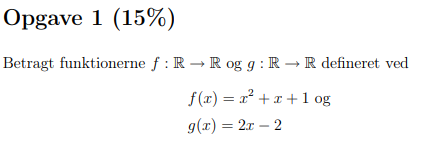
\includegraphics[scale=1]{Opgave1Formulering}
\end{figure}

Jeg vil bare gerne have det her ind i TKL00OpgSkriv D:

\end{document}
